
\documentclass[
  unknownkeysallowed %  ignore keyval errors (produced by Lato font)
]{beamer}

\usepackage[T1]{fontenc}
\usepackage[utf8]{inputenc}
\usepackage[spanish]{babel}

\usepackage{pgf,pgfpages}
\usepackage{tikz}
\usetikzlibrary{arrows,shapes,backgrounds,calc}
% Daniel's proposal for "uncovering" parts of a tikz-tree %
\tikzset{
  minimized/.style={scale=0.3},
  noshadowed/.style={opacity=1.0},
  shadowed/.style={opacity=0.4},
  invisible/.style={opacity=0},
  minimize on/.style={alt=#1{minimized}{}},
  visible on/.style={alt=#1{}{invisible}},
  shadow on/.style={alt=#1{shadowed}{noshadowed}},
  alt/.code args={<#1>#2#3}{%
    \alt<#1>{\pgfkeysalso{#2}}{\pgfkeysalso{#3}} % \pgfkeysalso doesn't change the path
  },
}

\usepackage{graphicx}
\usepackage{colortbl}
\usepackage{media9}

%% Beamer style.....
\mode<presentation>
{
  \usetheme{PHD}
  \setbeamercovered{transparent}
  \setbeamertemplate{items}[square]
}

%\usefonttheme[onlymath]{serif}

\beamertemplatenavigationsymbolsempty

\defbeamertemplate{enumerate item}{mycircle}
{
  %\usebeamerfont*{item projected}%
  \usebeamercolor[bg]{item projected}%
  \begin{pgfpicture}{0ex}{0ex}{1.5ex}{0ex}
    \pgfcircle[fill]{\pgfpoint{-0.1pt}{.65ex}}{1.1ex}
    \pgfbox[center,base]{\color{PHDyellow}{\insertenumlabel}}
  \end{pgfpicture}%
}
[action]
{\setbeamerfont{item projected}{size=\scriptsize}}
\setbeamertemplate{enumerate item}[mycircle]

%..............beamer style

\newcommand{\strip}[1]{%
  \begin{flushright}
    \color{PHDgrayC}
    \scriptsize{#1}
\end{flushright}}

\title[Cerebro virtual]
{¿Cómo modelar un cerebro virtual usando simulación numérica y redes neuronales?\vspace*{-0.5cm}}
\author[JRR, NOR, DAS]{%
  {J. Rafael Rodr\'{\i}guez Galv\'an\\
  Noelia Ortega Román\\
  Daniel Acosta Soba}
  \\[0.2em]
  {\small \em Grado en Matemáticas}
  \\[0.2em]
  {\scriptsize Puerto Real, 21/11/2023}
  \\[1em]
  
\includegraphics[width=2.5em]{img/cc-by}
}
\date{}

% XeLaTeX font choosing
% \usepackage{fontspec}%{xltxtra} %fontspec}
% \setsansfont{Fontin Sans}
% \setsansfont{Lato}

% PDFLaTeX font choosing
\usepackage[default, scale=1.0]{lato}
% \usepackage[math, default, scale=1.0]{lato}
% \usepackage[math, default, scale=0.95]{vollkorn}

% Different math fonts, see http://tug.org/pracjourn/2006-1/hartke/hartke.pdf
%\usepackage{eulervm}
%\usepackage{ccfonts, eulervm}
%\usepackage[math]{kurier}
%\usepackage[math]{anttor}
%\usepackage{pxfonts}
%\usepackage{mathpazo}
%\usepackage{mathpple}
%\usepackage[varg]{txfonts}
%\usepackage{arev}
%\usepackage{fourier}

\usepackage{tabularx}
\usepackage{array, multirow, booktabs, rotating} % booktabs: toprule, midrule...



%\newtheorem{remark}{Remark}
%\newtheorem{theorem}{Theorem}

\definecolor{OBcolor}{rgb}{0.2, 0.2, 0.8}
\newcommand\gris{\color{PHDgray}}
\newcommand\amarillo{\color{PHDyellow}}
\newcommand\video[2][0.8\textheight]{% #1: file #2: height
  \includemedia{\framebox[\linewidth]{\rule{0pt}{#2}}}{#1}
  \par\hfill\scriptsize Vídeo: #1
}
\newcommand{\llaveizq}[1]{$\left\{
  \begin{tabular}{@{}l@{}}#1\end{tabular}\right.$}
\newcommand{\llaveder}[1]{$\left.
  \begin{tabular}{@{}l@{}}#1\end{tabular}\right\}$}

\setcounter{tocdepth}{1}

%%%%%%%%%
% Vídeo
%%%%%%%%%

\usepackage{movie15}

\newcommand{\playVideoMovie}[3]{%
  \includemovie[autoplay,
  controls, % Show Play/Stop buttons
  ]{#1}{#2}{#3}}

%%%%%%%%%
% Colors
%%%%%%%%%

\definecolor{lightred}{RGB}{255,210,202}
\definecolor{lightblue}{HTML}{EEF4F8}
\definecolor{lightgreen}{HTML}{F6FFE6}
\definecolor{bananamania}{rgb}{0.98, 0.91, 0.71}

%%%%%%%%%
% Macros
%%%%%%%%%

\def\WW{\boldsymbol{W}}
\def\bb{\boldsymbol{b}}
\def\yy{\boldsymbol{y}}
\def\xx{\boldsymbol{x}}

%======================================================================
\begin{document}
%======================================================================

%
% Portada ............................................................
%
\setbeamertemplate{background}
 {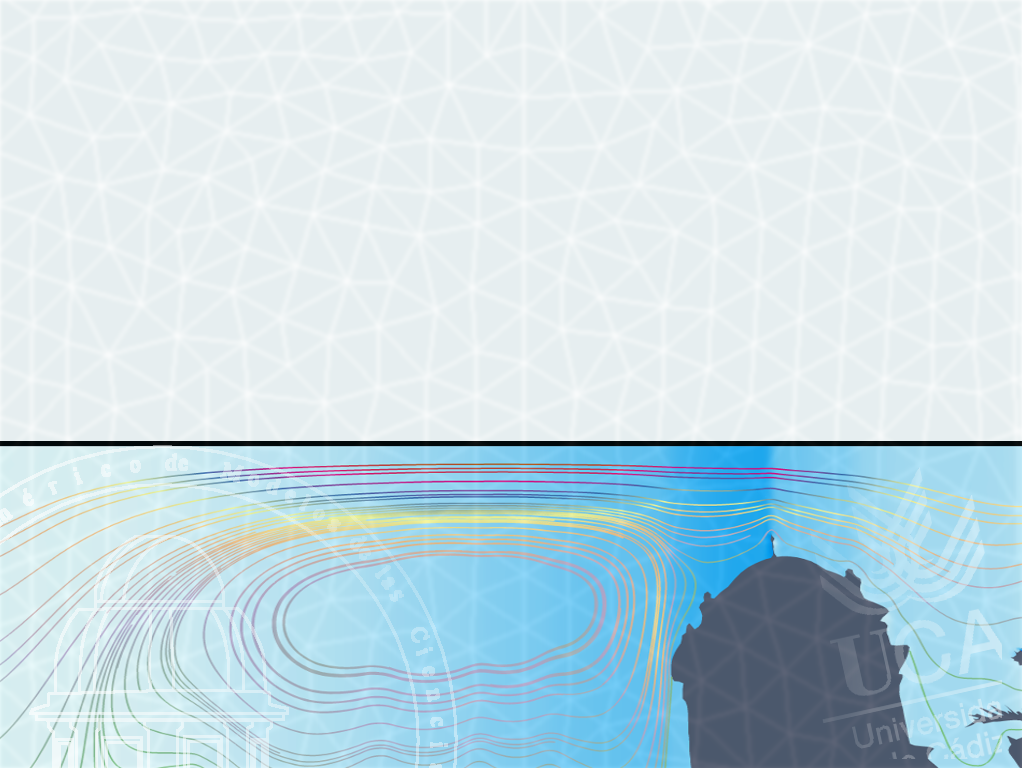
\includegraphics[width=\paperwidth,height=\paperheight]{frontpage_bg}}
\setbeamertemplate{footline}[default]

% Write custom titlepage ------->>>
\begin{frame}
  \titlepage
  \vspace{2.5cm}
\end{frame}

%
% Contenidos ............................................................
%

% Set the background for the rest of the slides.
\setbeamertemplate{background}
 {
\includegraphics[width=\paperwidth,height=\paperheight]{slide_bg}}

% \begin{frame}{Plan}
%   \tableofcontents
% \end{frame}

\section{Introducción}

\begin{frame}{El <<mundo de las ideas>> y <<mundo real>>}
  \begin{minipage}{0.45\linewidth}
    \vspace{-1.5em}
    % \begin{tikzpicture}
    %   \draw
    %   (3,-1) coordinate (a) node[right] {a}
    %   -- (0,0) coordinate (b) node[left] {b}
    %   -- (2,2) coordinate (c) node[above right] {c}
    %   pic["$\alpha$", draw=orange, <->, angle eccentricity=1.2, angle radius=1cm]
    %   {angle=a--b--c};
    % \end{tikzpicture}
    $$
    (a-b)(a+b)=a^2-b^2 \qquad
    $$
    \begin{center}
      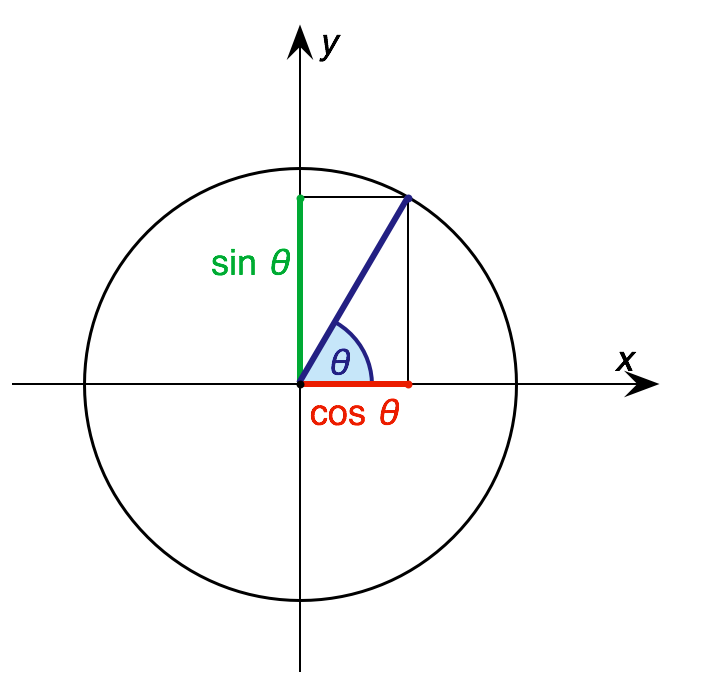
\includegraphics[width=0.65\linewidth,height=0.6\linewidth]{img/sin-cos}
    \end{center}
    \vspace{-1em}
    \begin{align*}
    \int_a^b f(x) \; dx = F(b)-F(a)
      \\[2em]
      \small
      \left\{
      \begin{aligned}
        \frac{\partial \mathbf{u}}{\partial t} - \nu \Delta \mathbf{u}
        + \nabla p &= \mathbf{f} \quad \text{en } \Omega\subset\mathbb{R}^n,
        \\
        \nabla\cdot \mathbf{u} &= 0 \quad \text{en } \Omega\subset\mathbb{R}^n.
      \end{aligned}
                                 \right.
    \end{align*}
  \end{minipage}
  \quad
  \begin{minipage}{0.45\linewidth}
    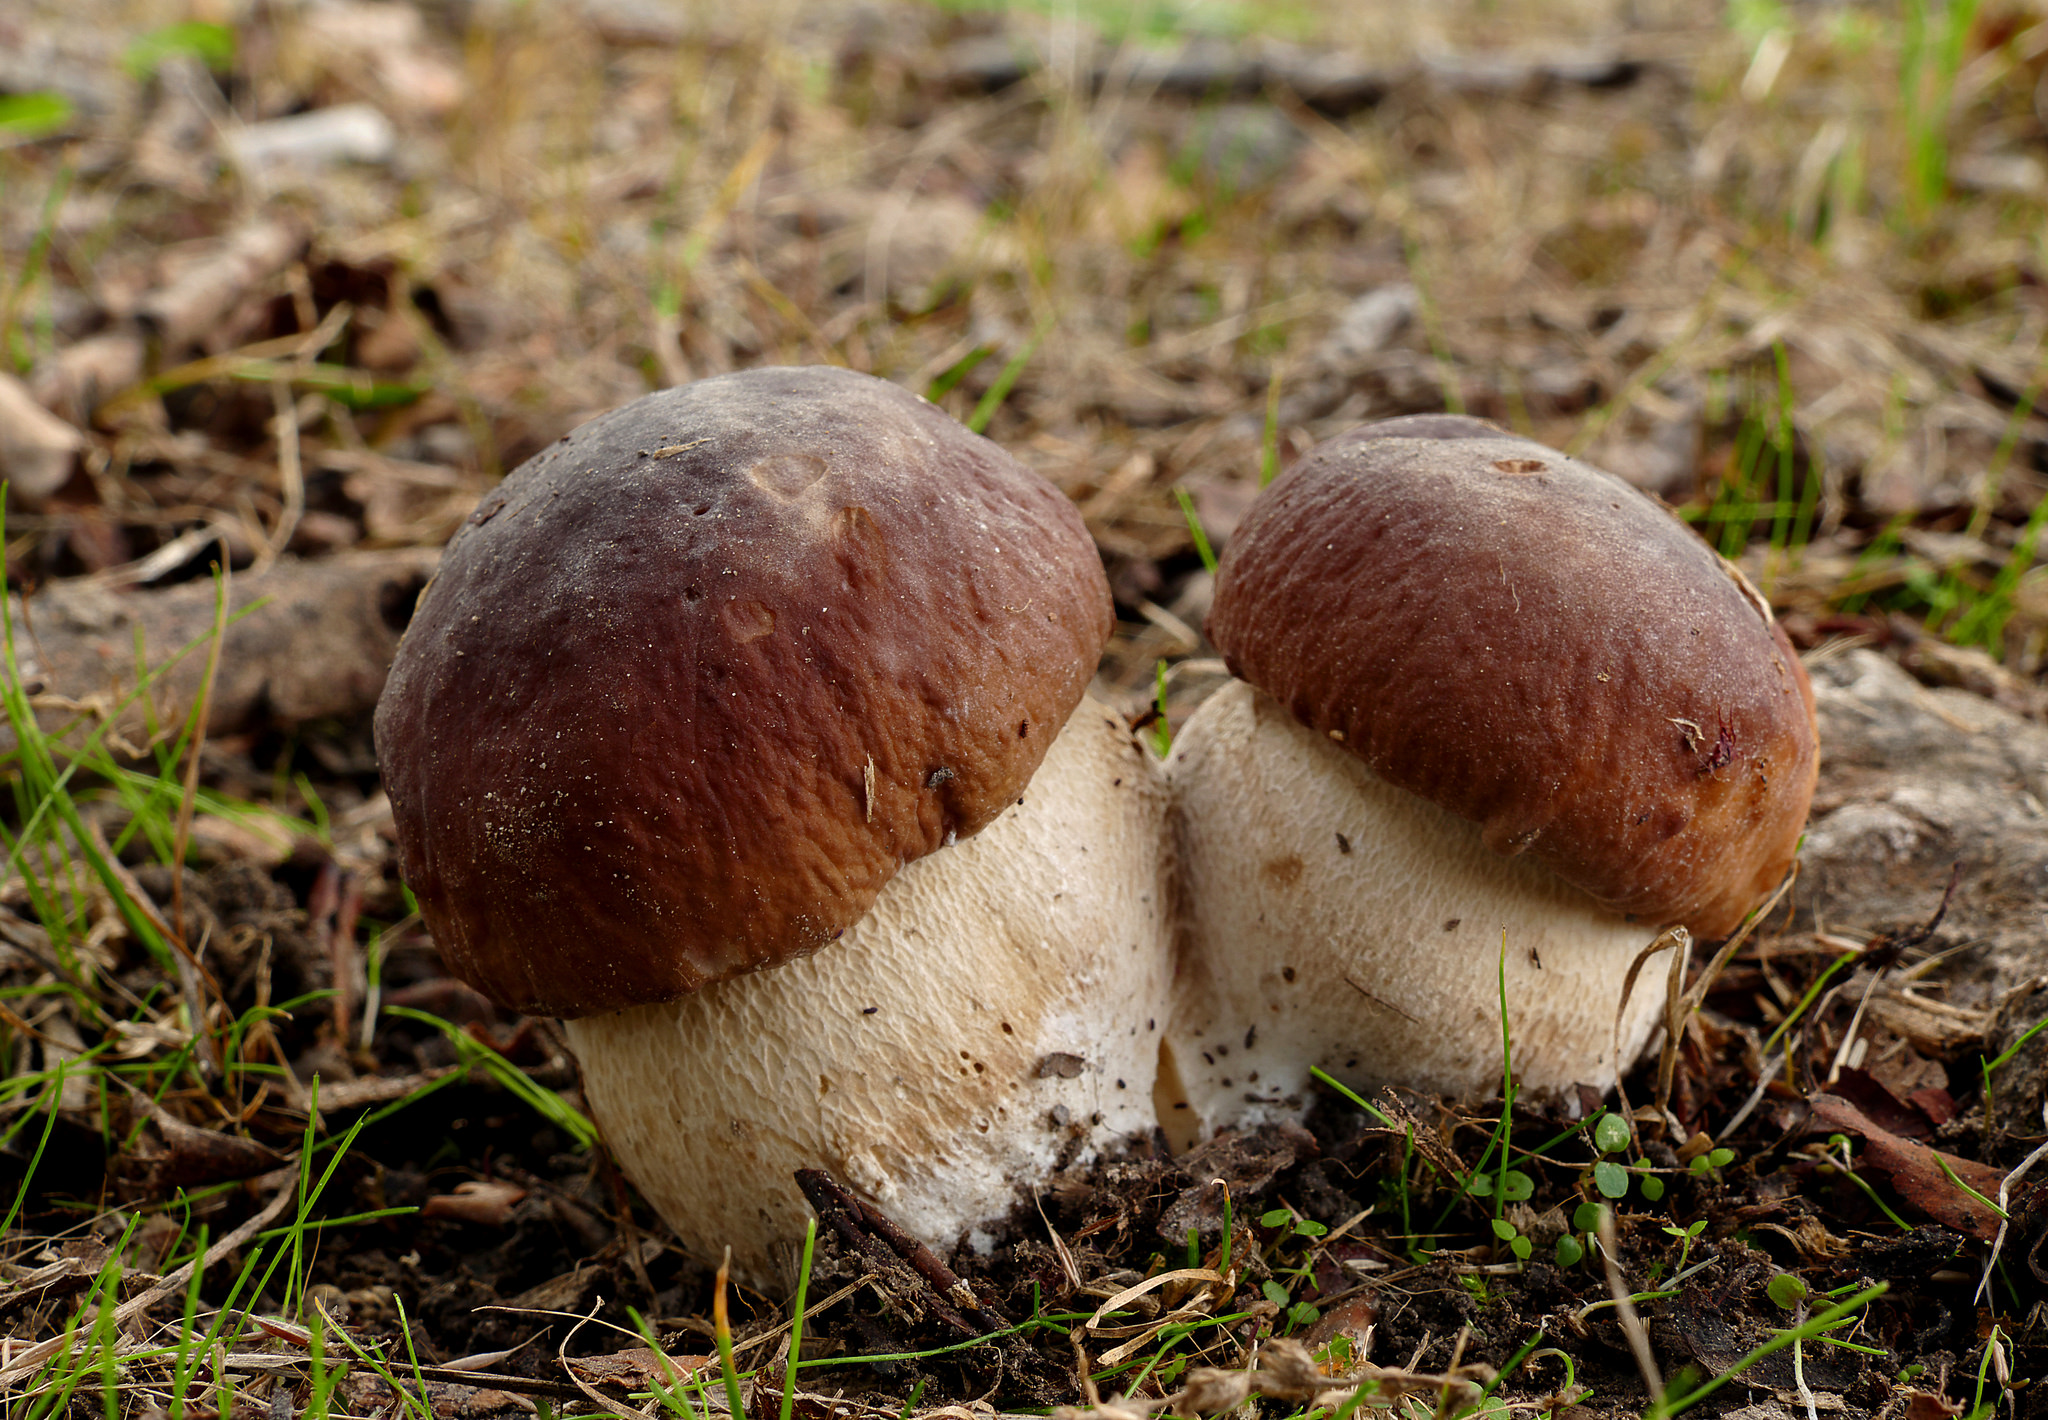
\includegraphics[width=0.8\linewidth]{img/setas}
    \\[-1.5em]
    \hspace*{2em}%
    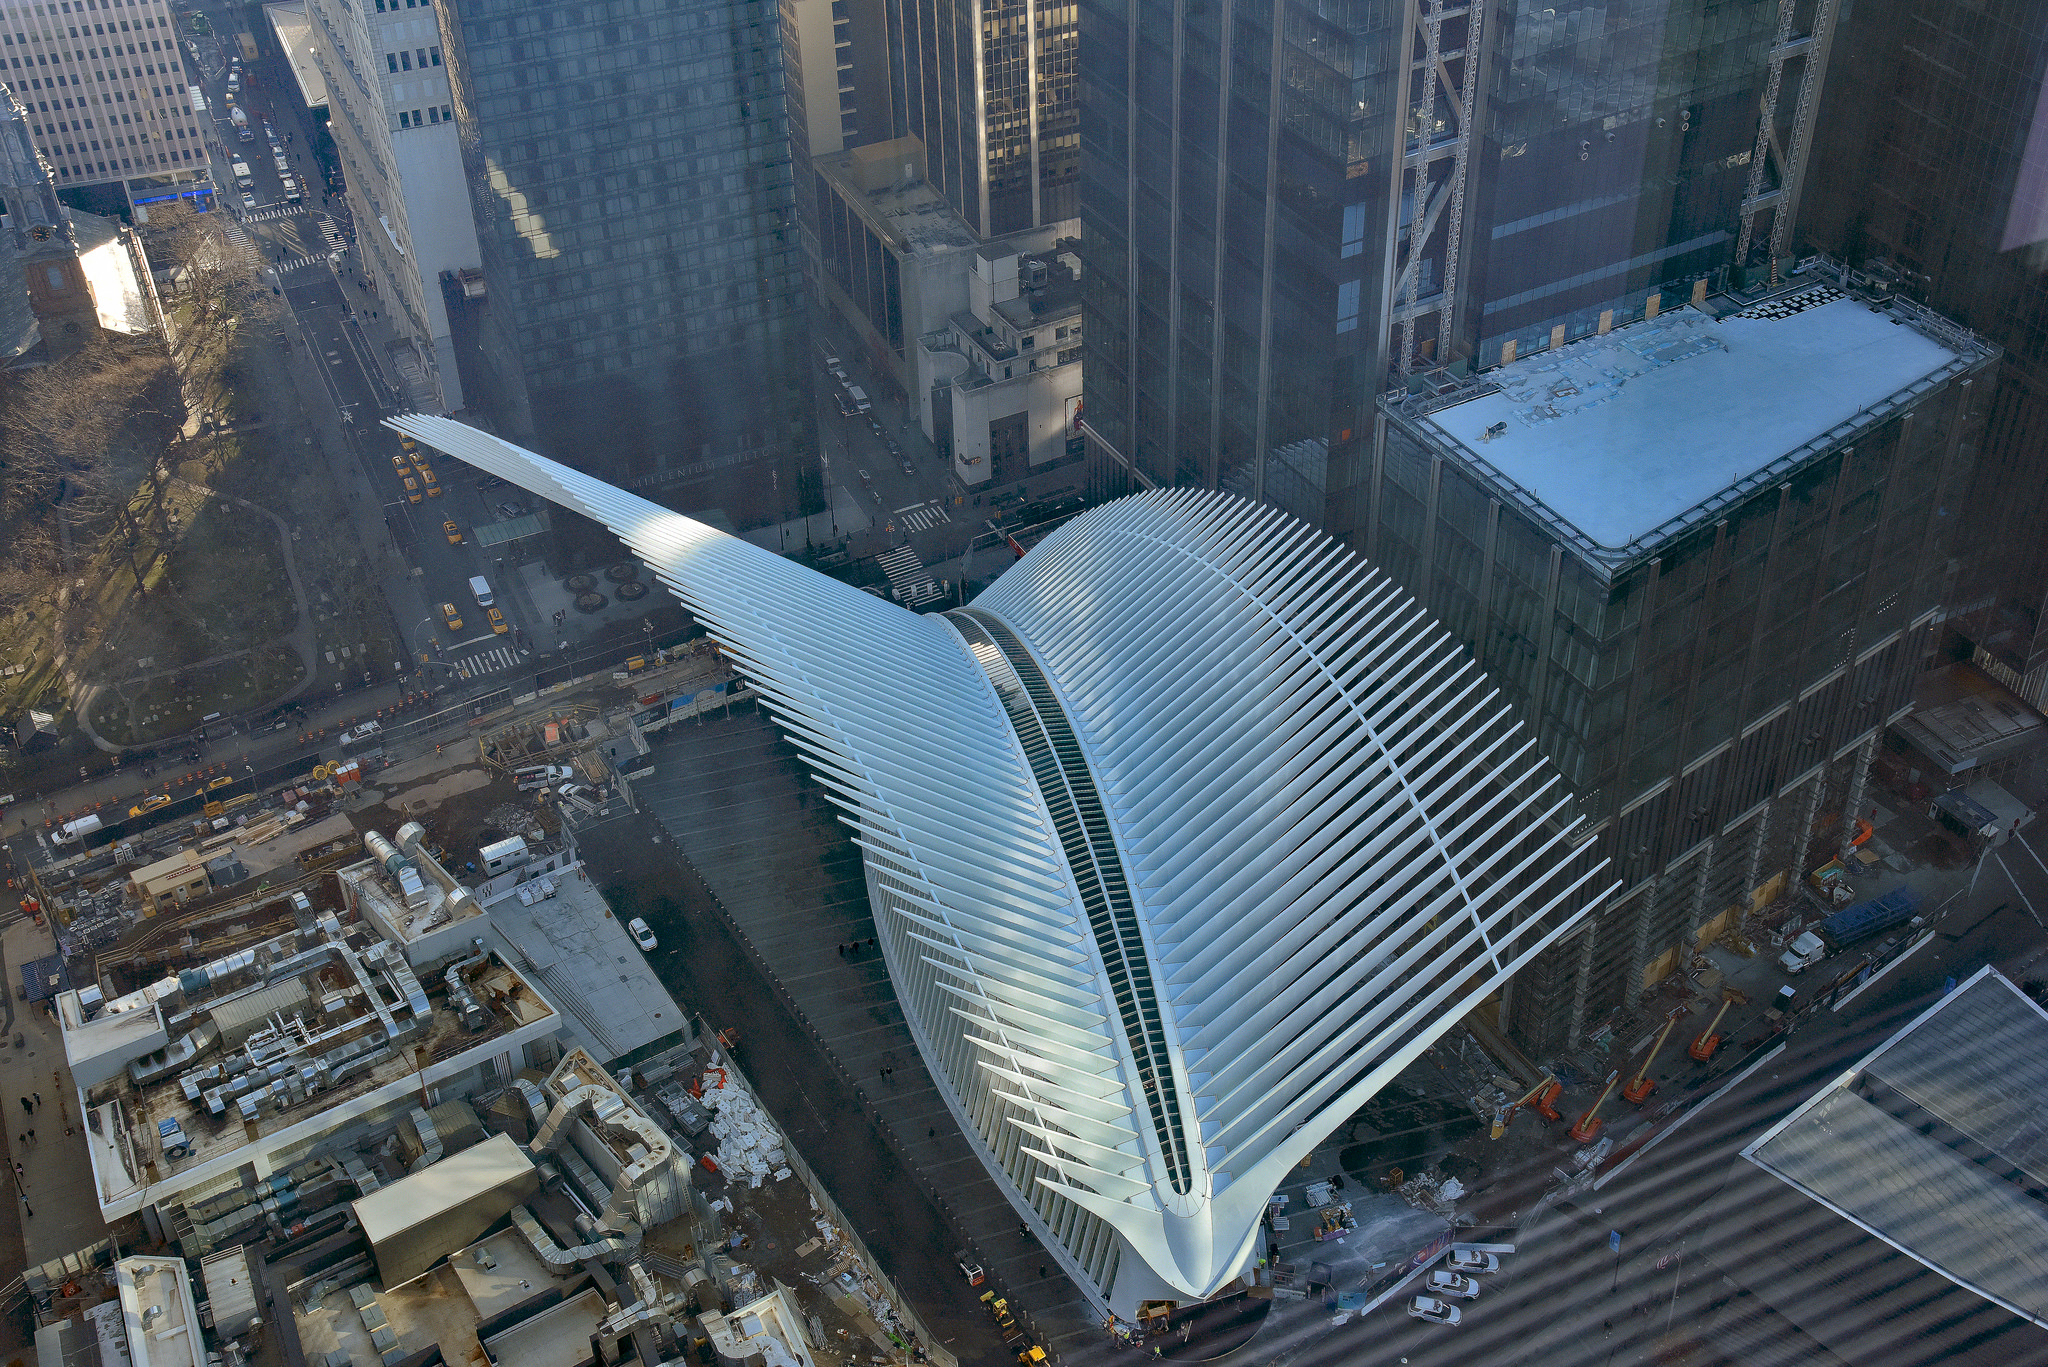
\includegraphics[width=0.8\linewidth]{img/world-trade-center}
    \\[-1em]
    \hspace*{3.5em}%
    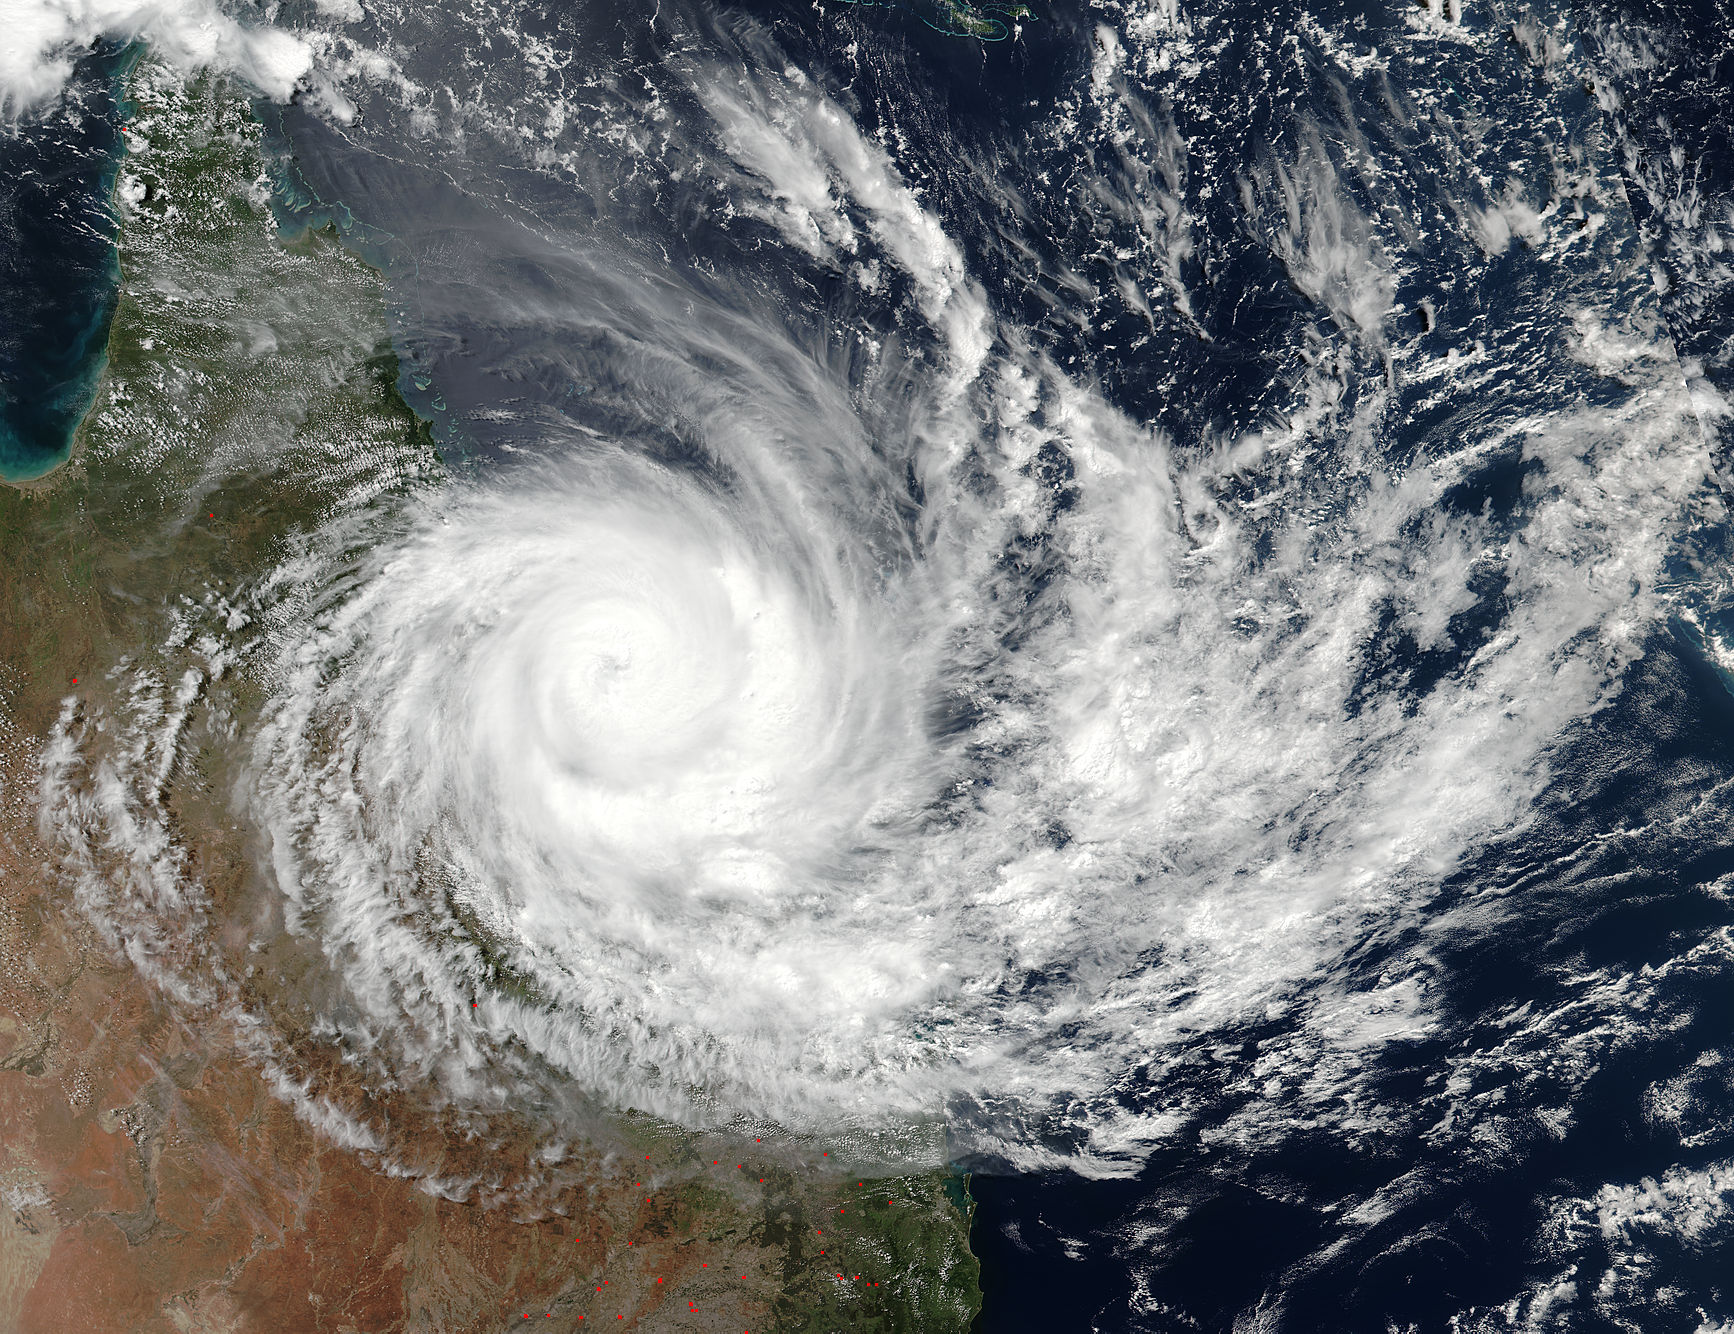
\includegraphics[width=0.8\linewidth]{img/ciclon}
  \end{minipage}
  \begin{minipage}{0.45\linewidth}
  \end{minipage}
\end{frame}

\begin{frame}{Internet...}
    \begin{center}
      \begin{tikzpicture}
        \node[shadow on=<2->] {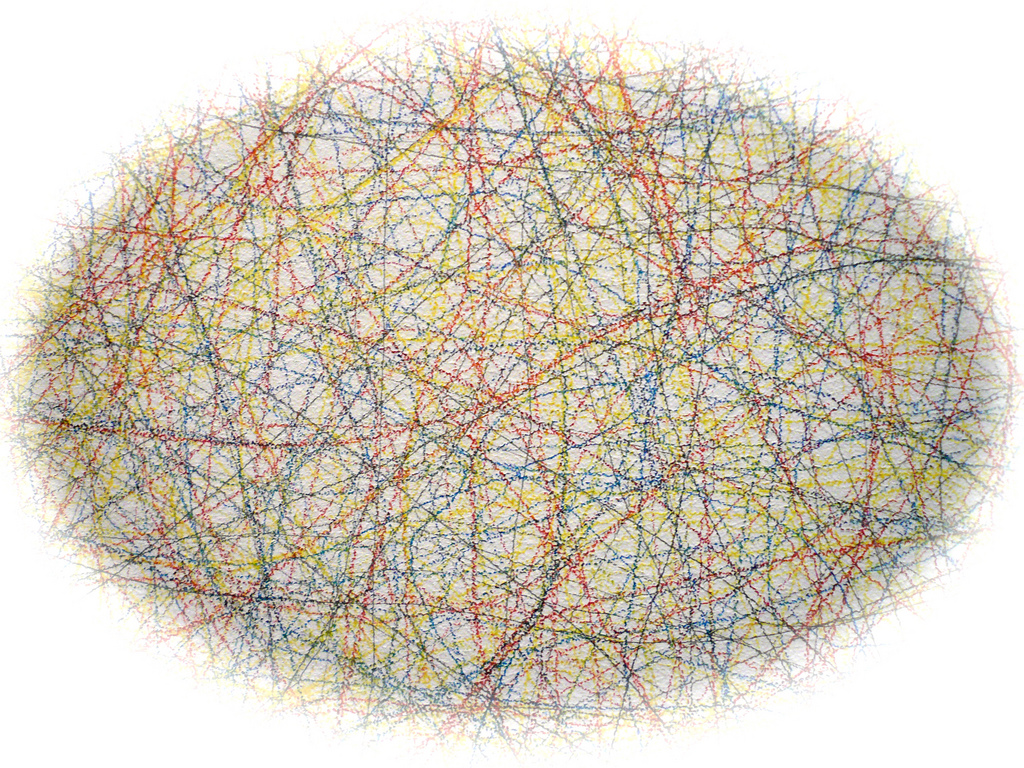
\includegraphics[width=0.83\linewidth]{img/internet}};
        \node<2-> at (0,1.5) {\textbf{4,498,700,644} usuarios en el
          mundo\footnote{\color{gray}Datos recogidos el 10/3/2020 de
            \url{http://www.internetlivestats.com}}};
        \node<2-> at (0,0.6) {\textbf{1,755,452,943} sitios web\footnotemark[\value{footnote}]};
        \node<3> at (0, -0.6) {{\large\emph{...¿cómo encuentras la}}};
        \node<3> at (0, -1.4) {{\LARGE\emph{\textbf{\alert{información que te interesa}}}}};
        \node<3> at (0, -2.3) {{\Huge\emph{\textbf{?}}}};
      \end{tikzpicture}
    \end{center}
\end{frame}

\begin{frame}{Buscadores web}
  \vspace*{-1em}
  \begin{flushright}
    \begin{tikzpicture}
      \node[minimize on=<2-3>] {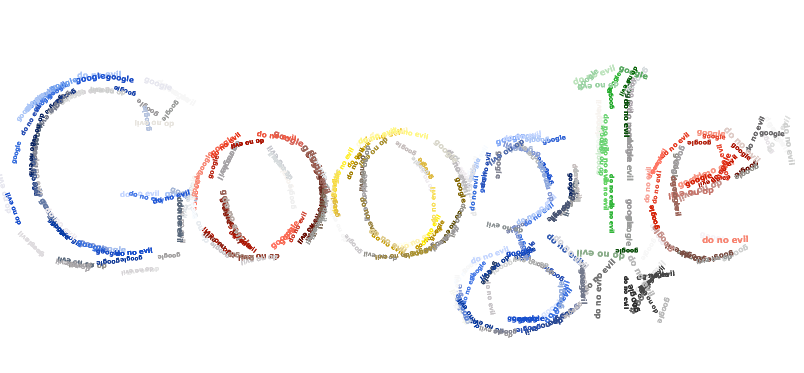
\includegraphics[width=0.9\linewidth]{img/google}};
    \end{tikzpicture}
  \end{flushright}
  \vspace*{-4.9em}
  \begin{flushleft}
    \begin{tikzpicture}
      \node<2->[minimize on=<4>] {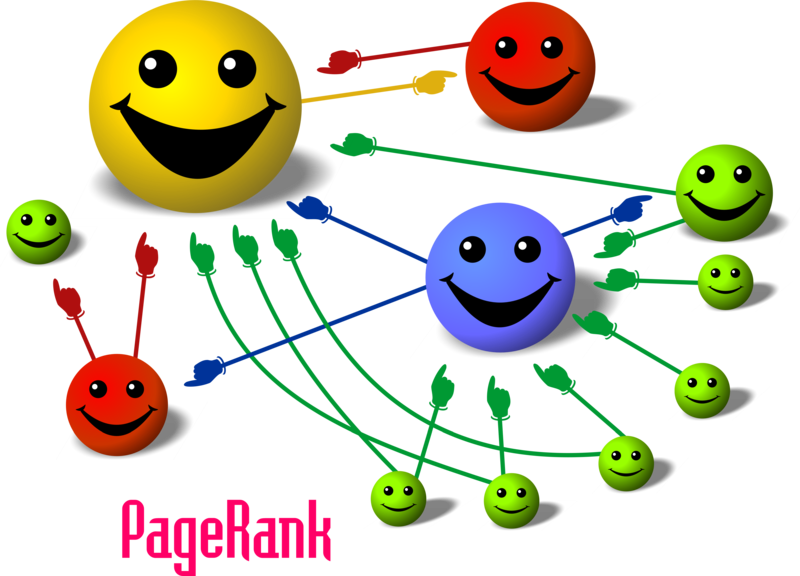
\includegraphics[width=0.6\linewidth]{img/page-rank}};
      \node<2-3> at (5.5,-1.9) {\large \it {\bfseries\href{https://es.wikipedia.org/wiki/Algoritmo}{\structure{Algoritmo}}} <<PageRank>>};
      \node<2-3> at (4.05,-3.0) {\small $PR(A) = {1 - d \over N} + d \left( \frac{PR(B)}{L(B)}+ \frac{PR(C)}{L(C)}+ \frac{PR(D)}{L(D)}+\,\cdots \right)$};
      \node<3> at (2.1,-4.1) {\textbf{Enorme \textit{sistema de ecuaciones}}: ¡una incógnita por cada sitio web!};
      \node<3> at (3.5,-4.6) {\small\color{gray}...aunque existen métodos eficientes para resolverlos};
      \node<4> at (5.2,-1.3) {
        \begin{tabular}{c}
          \large
          !El \textit{éxito de los buscadores web} se basa en las
          \\[1.2em]
          \Huge \textbf{matemáticas}!
        \end{tabular}
      };
    \end{tikzpicture}
  \end{flushleft}
\end{frame}

\begin{frame}
  \Large
  \begin{center}
    ~
    \\[2em]
    En la vida diaria
    \\[1.5em]
    hay muchas más \ \alert{\LARGE m a t e m á t i c a s}
    \\[1.5em]
    de lo que se podría pensar.
    \\[4em]
    \small
  \onslide<2>{\href{http://www.cedya2017.org/sesiones_especiales.html}{Sesiones especiales en el congreso <<XXV CEDYA / XV CMA>>}}
  \end{center}
\end{frame}

\begin{frame}{Modelos matemáticos}
  \begin{center}
      \begin{tikzpicture}[
        % Define standard arrow tip
        >=stealth',
        % Define style for boxes
        punkt/.style={
           rectangle,
           rounded corners,
           scale=1.1, fill=gray!20,
           draw=black, very thick,
           text width=6.5em,
           minimum height=2em,
           text centered},
         % Define arrow style
         pil/.style={
           ->,
           very thick,
           color=black!75!blue,
           shorten <=2pt,
           shorten >=2pt},
         % line width=1.2pt
        ]
        \node[punkt] (A) at (0,0) {\color{PHDgreen}\em <<Mundo real>>};
        \node[punkt] (B) at (6,0) {\color{PHDred}\em Modelo matemático}
        edge[pil, <-, bend left=-45] node[above] {\footnotesize
          \begin{tabular}{l}Leyes de la naturaleza\end{tabular}} (A);
        \node[punkt] (C) at (3,-3) {\color{orange}\em Simulación en ordenador}
        edge[pil, ->, bend left=45]  node[left] {\footnotesize
          \begin{tabular}{l} $\bullet$ Validación\\$\bullet$ Predicción\end{tabular}} (A)
        edge[pil, <-, bend left=-45, inner sep=1.0ex, align=right] node[right] {\footnotesize
          \begin{tabular}{l} $\bullet$ Análisis\\$\bullet$ Aproximación numérica \\
            $\bullet$ Algoritmos\end{tabular}} (B);
        % \path[line width=1.2pt, ->] (A) edge (B);
        % \path[line width=1.2pt, ->] (B) edge (C);
        % \path[line width=1.2pt, ->] (C) edge (A);
      \end{tikzpicture}
  \end{center}
\end{frame}

\begin{frame}{Modelos climáticos}
  \begin{minipage}{0.55\linewidth}
    \begin{flushright}
      \onslide<1->{\color{darkgray}\small\emph{¿Cómo se comportan los fluidos que forman <<\structure{\bfseries atmósfera}>> y <<\structure{\bfseries océanos}>>?}}
    \end{flushright}
    \vspace{0.5em}
    \onslide<2->{
      \begin{flushright}
        {Modelo matemático (simplificado)
          \color{darkgray}\scriptsize(ecuaciones de
          Navier-Stokes)}
      \end{flushright}
      \begin{equation*}
        \left\{
          \begin{aligned}
            \frac{\partial \alert<4>{\mathbf{u}}}{\partial t}
            + (\mathbf{\alert<4>u}\cdot\nabla)\mathbf{\alert<4>u}
            - \nu \Delta \mathbf{\alert<4>u}
            + \nabla \alert<3>p &= \mathbf{f},
            \\
            \nabla\cdot \mathbf{\alert<4>u} &= 0.
          \end{aligned}
        \right.
      \end{equation*}
    }
    \vspace{0.1em}
    \begin{flushleft}
     \onslide<3>{\alert<3>{\bf P}resión atmosférica}
     \\[0.5em]
     \onslide<4>{\alert<4>{\bf V}elocidad del fluido}
     \\[0.5em]
     \onslide<5>{Análisis del modelo:}
     \\[0.3em]
     \hfill \onslide<5>{\footnotesize\color{darkgray}¿Existe solución? ¿Con qué características?}
   \end{flushleft}
  \end{minipage}
  \hfill
  \begin{minipage}{0.40\linewidth}
    \includegraphics<1-3>[width=0.9\linewidth,height=1.2\linewidth]{img/tiempo-atmosf}
    \includegraphics<4->[width=1.0\linewidth,height=1.2\linewidth]{img/modelos-tiempo-atmosf}
  \end{minipage}
\end{frame}

\begin{frame}{Aproximación numérica}
  \small
  \begin{center}
    \em
    Convertir un mundo de \structure{complejidad infinita} en un modelo
    \structure{finito-dimensional}
  \end{center}
  \begin{minipage}{0.45\linewidth}
    \begin{itemize}
    \item<2-> \alert{Aproximación del dominio de cálculo} (triangulación)
    \item<2-> Mejor cuanto más grande sea el número de triángulos!!
    % \item<3-> Aproximación numérica de de las ecuaciones
    \item<3-> Resolución de \alert{enormes sistemas de ecuaciones} (incógnitas en
      cada vértice)
    \end{itemize}
  \end{minipage}
  \hfill
  \begin{minipage}{0.5\linewidth}
    \includegraphics<1->[width=1.0\linewidth,height=0.65\linewidth]{img/malla-estrecho-2d}
  \end{minipage}
  \pause
  \vspace*{1em} \onslide<4>{
    Cientos de miles de incógnitas {\color{gray}\dotfill} \\[0.7em]
    {\color{gray}\dotfill} no linealidad {\color{gray}\dotfill} un mundo 3D {\color{gray}\dotfill}\\[0.7em]
    {\color{gray}\dotfill} \large
    ¡\textit{\bfseries\alert{supercomputación}}!}
\end{frame}

\begin{frame}{Modelo 3D de flujo de corriente en el estrecho}
  \playVideoMovie{\textwidth}{0.8\textheight}{video/gibraltar-tubes-3d-30s.mp4}
  \par\hfill\scriptsize Vídeo: gibraltar-tubes-3d-30s.mp4
\end{frame}

\begin{frame}{Tsunamis}
  \small
  \begin{itemize}
  \item Distintos fenómenos requieren distintos modelos
  \begin{flushright}
    \scalebox{.5}{
      \begin{tikzpicture}[
        % Define standard arrow tip
        >=stealth',
        % Define style for boxes
        punkt/.style={
           rectangle,
           rounded corners,
           scale=1.1, fill=gray!20,
           draw=black, very thick,
           text width=6.5em,
           minimum height=2em,
           text centered},
         % Define arrow style
         pil/.style={
           ->,
           very thick,
           color=black!75!blue,
           shorten <=2pt,
           shorten >=2pt},
         % line width=1.2pt
        ]
        \node[punkt] (A) at (0,0) {\color{PHDgreen}\em <<Mundo real>>};
        \node[punkt] (B) at (6,0) {\color{PHDred}\em Modelo matemático}
        edge[pil, <-, bend left=-45] node[above] {\footnotesize
          \begin{tabular}{l}Leyes de la naturaleza\end{tabular}} (A);
        \node[punkt] (C) at (3,-3) {\color{orange}\em Simulación en ordenador}
        edge[pil, ->, bend left=45]  node[left] {\footnotesize
          \begin{tabular}{l} $\bullet$ Validación\\$\bullet$ Predicción\end{tabular}} (A)
        edge[pil, <-, bend left=-45, inner sep=1.0ex, align=right] node[right] {\footnotesize
          \begin{tabular}{l} $\bullet$ Análisis\\$\bullet$ Aproximación numérica \\
            $\bullet$ Algoritmos\end{tabular}} (B);
        % \path[line width=1.2pt, ->] (A) edge (B);
        % \path[line width=1.2pt, ->] (B) edge (C);
        % \path[line width=1.2pt, ->] (C) edge (A);
      \end{tikzpicture}
      }
    \end{flushright}
  \item Los fenómenos de ``tipo ondulatorio'' (sonidos, tsunamis) requieren ecuaciones de distinta naturaleza (hiperbólicas)
  \item Un nuevo modelo (ecuaciones de aguas poco profundas)
  \item Utilizado para estudiar tsunamis anteriores o predecir futuros efectos
  \item Vídeo...
  \end{itemize}
\end{frame}

\begin{frame}{Tsunami frente al cabo de San Vicente}
  \playVideoMovie{\textwidth}{0.8\textheight}{video/tsunami2.mp4}
  \par\hfill\scriptsize \href{https://www.youtube.com/watch?v=DkGmz0na00g}{Vídeo: tsunami2.mp4}
\end{frame}

\begin{frame}{Matemáticas en Ingeniería}
  \playVideoMovie{\textwidth}{0.8\textheight}{video/vortices-von-karman.mp4}
  \par\hfill\scriptsize \href{https://www.youtube.com/watch?v=E1fPolQ-uTI}{Vídeo: Cuerpo circular sumergido, vórtices de Von Karman}.
\end{frame}

\begin{frame}{Matemáticas en Ingeniería}

  {\large\bf Vídeos del prof. A. Quarteroni}
  \bigskip
  \begin{itemize}\itemsep1em
  \item \href{https://youtu.be/8W4oFOymiyM?t=995}{\textbf{Ingeniería
        naval}: optimización en el diseño de la quilla de un barco}
  \item \href{https://youtu.be/8W4oFOymiyM?t=888}{Aerodinámica y
      Automóviles: diseño óptimo de coches \textbf{de Fórmula 1}}
  \item \href{https://youtu.be/8W4oFOymiyM?t=887}{Ingeniería areoespacial}
  \end{itemize}
\end{frame}

\begin{frame}{... y mucho más...}
  ...utilizando \textbf{el mismo tipo de modelos matemáticos}...
  \par\hfill ...se pueden tratar \alert{\bf fenómenos completamente diferentes}...
  \bigskip
  \begin{itemize}\itemsep1em
  \item Matemáticas para la \textbf{\alert{economía}}
    \par\bigskip
    Material divulgativo del prof. Carlos Vázquez Cendón:

    \begin{itemize}\itemsep0.5em
    \item
      \href{http://www.unir.net/empresa/revista/noticias/matematicas-para-la-economia/549201449354/}{\em
        <<Las matemáticas son el lenguaje con el que se puede escribir
        con cierto rigor los modelos de la economía>>}
    \item
      \href{http://www.rtve.es/alacarta/audios/eureka/eureka-se-pudo-haber-previsto-crisis-matematicas-31-05-13/1847482}{\em
        ¿Se pudo haber previsto la crisis con matemáticas?}
      \par\smallskip\hfill {\em Análisis del riesgo financiero}
    \end{itemize}
  \item Matemáticas para videojuegos
  \item ...
  \item ... o \textbf{\alert{matemáticas en ciencias de la vida} {\Large !}}
  \end{itemize}
\end{frame}


\begin{frame}{Ciencias de la vida}
  \small

  {\normalsize\bf Flujo de sangre} (Vídeos de A. Quarteroni)
  \begin{itemize}
  \item \href{https://youtu.be/8W4oFOymiyM?t=511}{<<Las
      \textbf{Matemáticas} son nuestro \textbf{laboratorio
        inmaterial}>>}
  \item \href{https://youtu.be/8W4oFOymiyM?t=645}{\textit{Flujo de sangre} y deformación de la \textbf{arteria} carótida}
  \item \href{https://youtu.be/8W4oFOymiyM?t=787}{Diseño de \textit{bypasses} o \textbf{puentes coronarios}}
  \item \href{https://youtu.be/8W4oFOymiyM?t=823}{Entender cómo funciona el \textbf{cerebro humano}}
  \end{itemize}
  \smallskip
  {\normalsize\bf Oncología Matemática}:
  \begin{itemize}
  \item \href{https://es-es.facebook.com/recaida0/}{Recaída 0} (leucemia infantil)
  \item
    \href{http://matematicas.uclm.es/imaci/molab/mathoncol}{Laboratorio
      de Oncología Matemática, UCLM}
    \begin{quotation}\scriptsize\em
      <<Mathematical Oncology intends to \textbf{describe processes in oncology}
      using the tools and systematization methods of mathematics. This
      includes mainly \textbf{mathematical model} building and techniques from
      applied mathematics: differential equations, numerical methods,
      optimization, etc.

      The ultimate goals are to use that knowledge to \textbf{improve the
      current treatments of cancer} patients and to raise hypothesis
      that can be tested by clinicians and biologists. Thus unlike
      pure mathematics that is interested in the abstract objects in
      themselves we try to generate knowledge of direct applicability
      in Medicine.>>
    \end{quotation}
  \end{itemize}
  \smallskip
  {\large\bf Regeneración de \alert{lesiones cerebrales}...}
\end{frame}

% \begin{frame}{Ciencias de la vida}
%   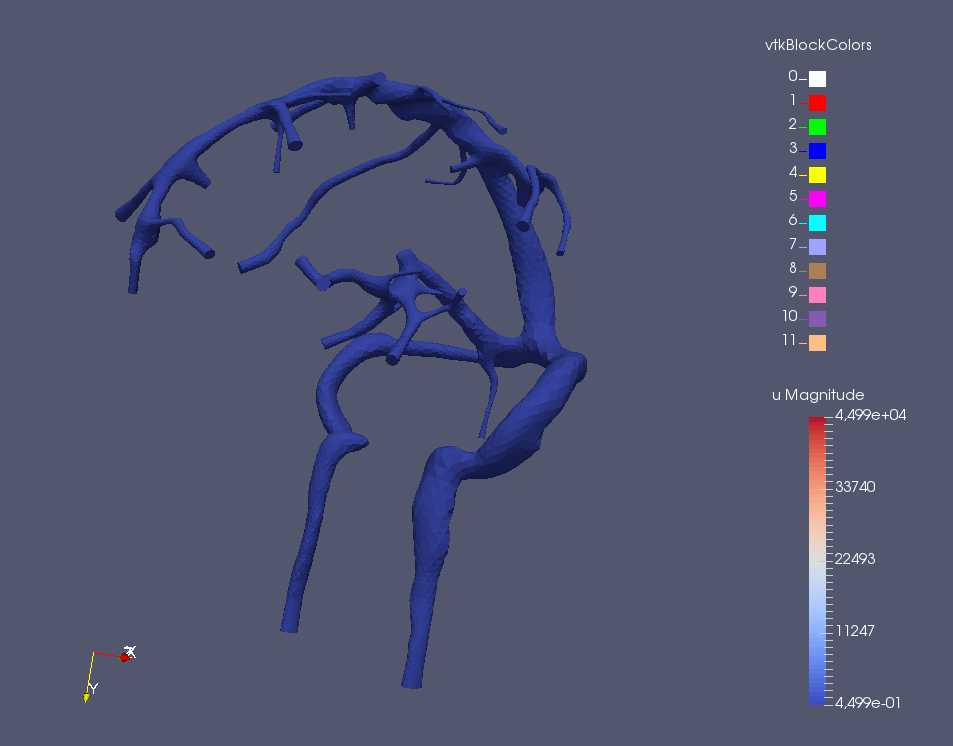
\includegraphics[width=0.8\linewidth]{img/brain}
%   \\
%   \textbf{Venas} en el \alert{\textbf cerebro humano}
% \end{frame}

\begin{frame}{Lesiones cerebrales y \textbf{neurogénesis}}
  \structure{Enfermedades neurológicas}:
  \begin{itemize}
  \item Principal causa de discapacidad... \par\smallskip
    ... y segunda causa de mortalidad en el mundo
  \item Su peso va en aumento, por el envejecimiento de la población
  \end{itemize}
  \bigskip
\textbf{\structure{Neurogénesis}}:  una prometedora oportunidad
\begin{itemize}
\item Mecanismo por el que se originan \textbf{neuroblastos}, células precursoras de neuronas
\item Tras nacer, siguen una ruta hacia el \textbf{bulbo olfatorio} (\structure{OB})
\item También se dirigen a \textbf{lesiones cerebrales}: una posibilidad para su curación
\end{itemize}
\end{frame}

\begin{frame}{Proyecto de investigación}
  \vspace{2em}
  \begin{center}
    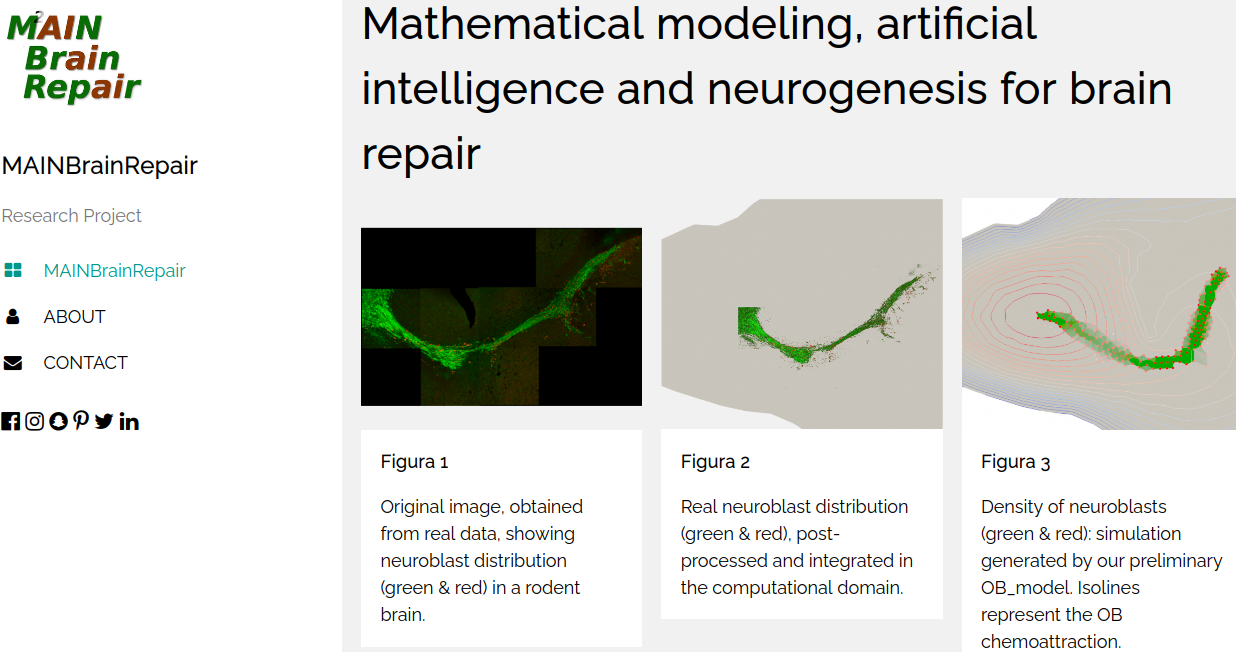
\includegraphics[width=1.0\linewidth]{img/MAINBrainRepair}
\end{center}
\begin{flushright}
  \scriptsize
  \url{https://mainbrainrepair.github.io/}
\end{flushright}
\end{frame}

\begin{frame}{Distribución de neuroblastos en el cerebro de un roedor}
  \medskip
  \begin{center}
    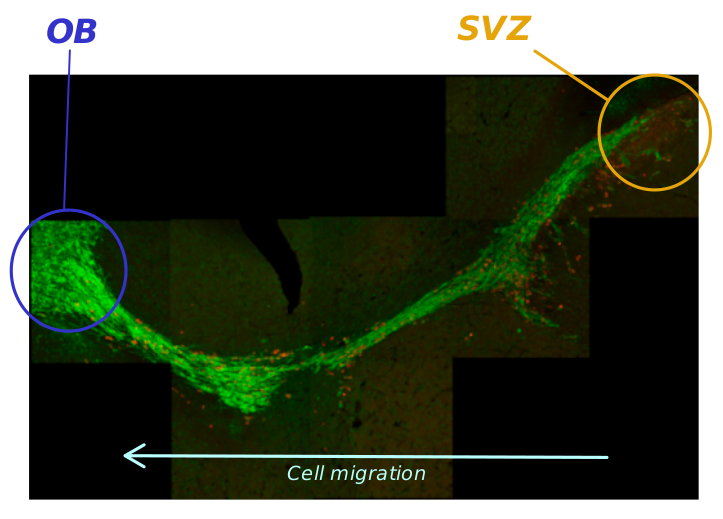
\includegraphics[width=0.8\linewidth]{img/neuroblastos-roedor-anotado}
  \end{center}
\end{frame}

\begin{frame}{Modelización matemática: quimiotaxis}
  \textbf{Quimiotaxis}
  \begin{quote}
    \small
  \em «Fenómeno en el que organismos
  unicelulares (\alert<1>{células}) o pluricelulares dirigen sus movimientos como respuesta a un
    \structure<1>{estímulo químico}»
\end{quote}

\bigskip
Ecuaciones de Keller-Segel (sistema de EDP)...
\par\hfill
...hallar \llaveizq{$u(x,t)$, \alert<1>{\textbf{densidad de células}} en $(x,t)$
  \\[0.2em]
  $v(x,t)$, \structure<1>{estímulo químico} tales que:}
\begin{align*}
  \alert<1>{u_t - \Delta u + \mathcal{X}\; \alert<2>{\nabla\cdot (u \structure<1-2>{\nabla v})} = 0},&
  \\
  \structure<1>{v_t - \Delta v + v - \alert<1>{u} = 0},&
  \\
  {\color{gray}+ \text{ condiciones iniciales }}&\text{\color{gray}y de contorno.}
\end{align*}
\vspace{-1.5em}
\begin{itemize}
\item <2> Término de \alert{quimioatracción} de $u$ hacia $\nabla v$ !!!
  \begin{itemize}
  \item $\mathcal{X}>0$, amplitud de la quimioatracción
  \end{itemize}
\item <2> Retos:
  \begin{itemize}
  \item Análisis matemático (explosión en tiempo finito)
  \item Aproximación numérica (EDP de tipo parabólico/\alert{hiperbólico} !!)
  \end{itemize}
\end{itemize}
\end{frame}

\begin{frame}{Modelo de migración de neuroblastos hacia OB}
  \vspace{-0.8em}
  \begin{overprint}
    \onslide<1>\centering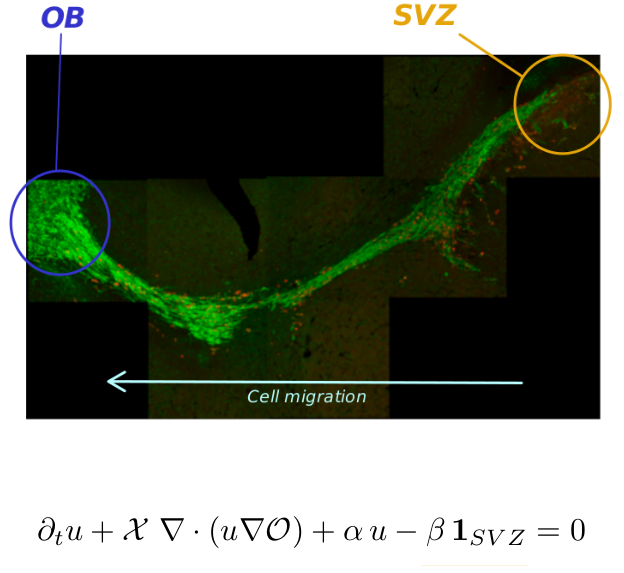
\includegraphics[width=0.64\linewidth]{img/ecuacion_nb_OB-0.png}
    \onslide<2>\centering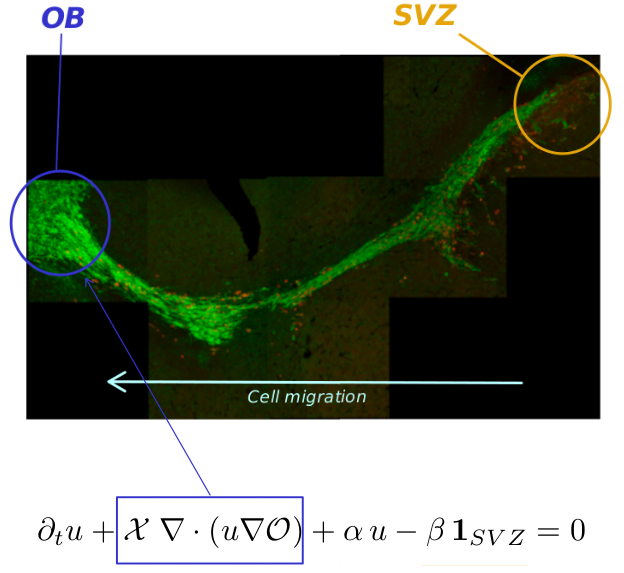
\includegraphics[width=0.64\linewidth]{img/ecuacion_nb_OB-1.png}
    \onslide<3->\centering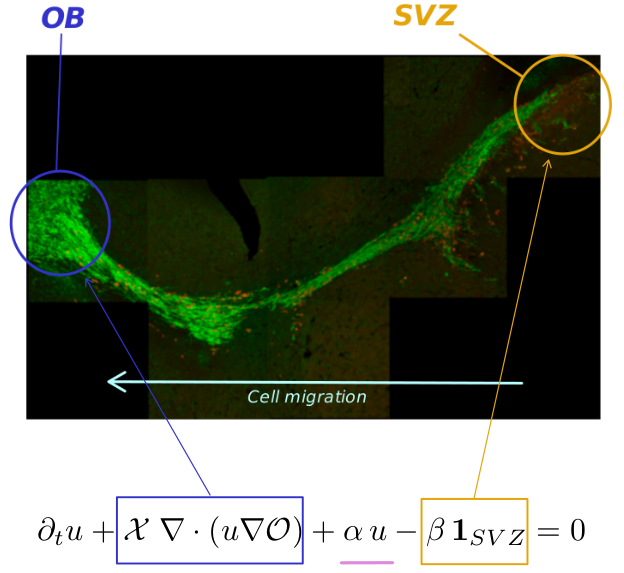
\includegraphics[width=0.64\linewidth]{img/ecuacion_nb_OB-2.png}
  \end{overprint}
  \bigskip
  \begin{itemize}\itemsep0.2em
  \item<2-> $\mathcal{O}(x)$: función «atracción química» por {\color{OBcolor}\textbf{\textit{OB}}}
  \item<3-> Parámetros: $ \mathcal{X}$, $\alpha$, $\beta$, «forma de $\mathcal{O}(x)$»
    \onslide<4>{\alert<4>{... \textbf{anisotropía}~\includegraphics<4>[height=\baselineskip]{img/icons8-innovation-64}}}
  \end{itemize}
\end{frame}

\begin{frame}{Resolución numérica}
    \textbf{Discretización en \alert{tiempo}}: método de Euler (Implícito)
    \begin{equation}
    u^{n+1} = u^n - \Delta t \cdot \big( \mathcal{X}\,\nabla\cdot(u^{n+1} \nabla\mathcal{O})
    + \alpha u^{n+1} -\beta \mathbf{1}_{SVZ} \big)
    \label{eq:1}
  \end{equation}

  \textbf{Discretización en \alert{espacio}}: método de Galerkin (Discontinuo)
  \par\medskip
    \begin{tabular*}{\linewidth}{ll}
      \begin{minipage}{0.66\linewidth}
        \small
        \begin{itemize}
        \item Mallado del dominio espacial
        \item Aproximación ``$P0$'' de la solución: polinomios de grado $m=0$ en cada triángulo
        \item Multiplicamos~(\ref{eq:1}) por funciones test (en triángulos) en integramos por partes.
          \begin{itemize}
          \item Saltos (flujos) en las aristas
        \end{itemize}
      \item En cada etapa de tiempo, resolución de un gran sistema de ecuaciones.
        \begin{itemize}
        \item Incógnitas: solución en cada triángulo
      \end{itemize}
        \end{itemize}
      \end{minipage}
      &
        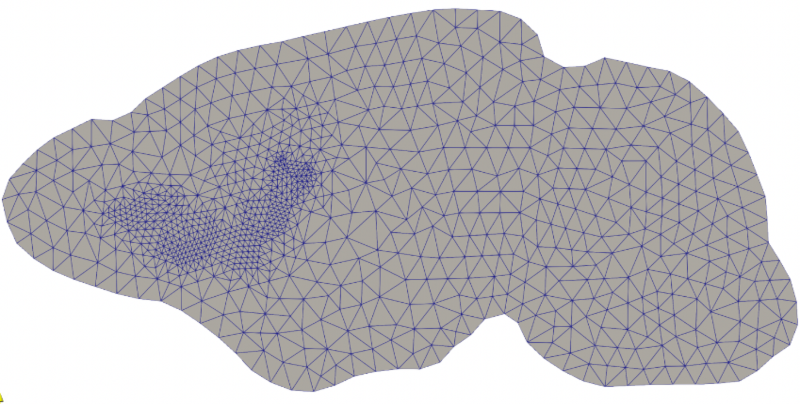
\includegraphics[width=0.31\linewidth]{img/brain_mesh}
    \end{tabular*}
\end{frame}

% #################### REDES NEURONALES #####################

\begin{frame}{¿Qué son las redes neuronales?}
  \begin{itemize}
    \item<1-> Herramienta de \structure{inteligencia artificial}:
    \begin{itemize}
      \item Aprendizaje supervisado.
      \item Deep learning.
    \end{itemize}
    \item<2-> Desde un punto de vista matemático: \structure{composición de funciones dependientes de parámetros}.
  \end{itemize}
  \begin{figure}
    \centering
    \begin{tikzpicture}[scale=0.8, every node/.style={scale=0.75}, square/.style={regular polygon,regular polygon sides=4}]
      \draw[fill=lightred, draw=white] (1,-1.7) rectangle (-1,1.7);
      \draw[fill=lightblue, draw=white] (7,-2.2) rectangle (2,2.2);
      \draw[fill=lightgreen!95!black, draw=white] (10,-0.7) rectangle (8,0.7);

      \node[fill=white] at (0,1) [draw, square] (x1) {$x_1$};
      \node[fill=white] at (0,0) [draw, square] (x2) {$x_2$};
      \node[fill=white] at (0,-1) [draw, square] (x3) {$x_3$};

      \node[fill=white] at (3,1.5) [draw, circle, inner sep=0.3cm] (hl1_1) { };
      \node[fill=white] at (3,0.5) [draw, circle, inner sep=0.3cm] (hl1_2) { };
      \node[fill=white] at (3,-0.5) [draw, circle, inner sep=0.3cm] (hl1_3) { };
      \node[fill=white] at (3,-1.5) [draw, circle, inner sep=0.3cm] (hl1_4) { };

      \node[fill=white] at (6,1.5) [draw, circle, inner sep=0.3cm] (hl2_1) { };
      \node[fill=white] at (6,0.5) [draw, circle, inner sep=0.3cm] (hl2_2) { };
      \node[fill=white] at (6,-0.5) [draw, circle, inner sep=0.3cm] (hl2_3) { };
      \node[fill=white] at (6,-1.5) [draw, circle, inner sep=0.3cm] (hl2_4) { };

      \node[fill=white] at (9,0) [draw, square] (y) {$\hat y$};

      \draw[-stealth] (x1) -- (hl1_1);
      \draw[-stealth] (x1) -- (hl1_2);
      \draw[-stealth] (x1) -- (hl1_3);
      \draw[-stealth] (x1) -- (hl1_4);

      \draw[-stealth] (x2) -- (hl1_1);
      \draw[-stealth] (x2) -- (hl1_2);
      \draw[-stealth] (x2) -- (hl1_3);
      \draw[-stealth] (x2) -- (hl1_4);

      \draw[-stealth] (x3) -- (hl1_1);
      \draw[-stealth] (x3) -- (hl1_2);
      \draw[-stealth] (x3) -- (hl1_3);
      \draw[-stealth] (x3) -- (hl1_4);

      \draw[-stealth] (hl1_1) -- (hl2_1);
      \draw[-stealth] (hl1_1) -- (hl2_2);
      \draw[-stealth] (hl1_1) -- (hl2_3);
      \draw[-stealth] (hl1_1) -- (hl2_4);

      \draw[-stealth] (hl1_2) -- (hl2_1);
      \draw[-stealth] (hl1_2) -- (hl2_2);
      \draw[-stealth] (hl1_2) -- (hl2_3);
      \draw[-stealth] (hl1_2) -- (hl2_4);

      \draw[-stealth] (hl1_3) -- (hl2_1);
      \draw[-stealth] (hl1_3) -- (hl2_2);
      \draw[-stealth] (hl1_3) -- (hl2_3);
      \draw[-stealth] (hl1_3) -- (hl2_4);

      \draw[-stealth] (hl1_4) -- (hl2_1);
      \draw[-stealth] (hl1_4) -- (hl2_2);
      \draw[-stealth] (hl1_4) -- (hl2_3);
      \draw[-stealth] (hl1_4) -- (hl2_4);

      \draw[-stealth] (hl2_1) -- (y);
      \draw[-stealth] (hl2_2) -- (y);
      \draw[-stealth] (hl2_3) -- (y);
      \draw[-stealth] (hl2_4) -- (y);

      \node at (0,-2) (capa_entrada) {\textcolor{lightred!70!black}{capa de entrada}};
      \node at (3,-2.5) (capa_oculta_1) {\textcolor{lightblue!60!black}{capa oculta 1}};
      \node at (6,-2.5) (capa_oculta_2) {\textcolor{lightblue!60!black}{capa oculta 2}};
      \node at (9,-1) (capa_salida) {\textcolor{lightgreen!70!black}{capa de salida}};
    \end{tikzpicture}
    \caption{Perceptrón multicapa.}
  \end{figure}
\end{frame}

\begin{frame}{¿Cómo se construye un perceptrón multicapa?}
  \begin{itemize}
    \item Datos de entrada y salida conocidos: $\alert{(x,y)}$.
    \item Parámetros:
    \begin{itemize}
      \item Matrices $\alert{W_i}$.
      \item Vectores $\alert{b_i}$.
      \item En general, $\alert{\theta}$ representa al conjunto de parámetros.
    \end{itemize}
    \item Función de activación $\alert{\sigma}$:
    \begin{itemize}
      \item \structure{Sigmoide}.
      \item \structure{Tanh}.
      \item \structure{ReLU}.
      \item \structure{Softmax}.
    \end{itemize}
  \end{itemize}
  \begin{figure}
    \centering
    \begin{tikzpicture}[scale=0.75, every node/.style={scale=0.7}]
      \draw (0.5,-0.5) rectangle (-0.5,0.5);
      \draw (3.5,0) ellipse (1.5 and 1);
      \draw (8,0) ellipse (1.5 and 1);
      \draw (14.5,-0.5) rectangle (13.5, 0.5);

      \draw (4,0.94) -- (4,-0.94);
      \draw (8.5,0.94) -- (8.5,-0.94);

      \draw[-stealth](0.5,0) -- (2,0);
      \draw[-stealth] (5,0) -- (6.5,0);
      \draw[-stealth] (9.5,0) -- (11,0);
      \draw[-stealth] (12,0) -- (13.5,0);

      \node at (0,0) (x) {$x$};
      \node at (3,0) (hl1_1) {$W_1x+b_1$};
      \node at (4.5,0) (hl1_2) {$\sigma$};
      \node at (3.5,1.25) (hl1) {$\mathcal{N}_1$};
      \node at (7.5,0) (hl2_1) {$W_2\mathcal{N}_1+b_2$};
      \node at (9,0) (hl2_2) {$\sigma$};
      \node at (8,1.25) (hl2) {$\mathcal{N}_2$};
      \node at (11.5,0) (more) {$\cdots$};
      \node at (14,0) (out) {$\hat y$};

      % \node at (1.25,0.25) (W1) {$W_1$};
      %v\node at (3.75,0.25) (W2) {$W_1$};
      % \node at (6.25,0.25) (W3) {$W_3$};
    \end{tikzpicture}
    \caption{Composición de un perceptrón multicapa (\structure{forward propagation}).}
  \end{figure}
\end{frame}

\begin{frame}{~}
  \begin{figure}
    \centering
    \begin{tikzpicture}[scale=0.75, every node/.style={scale=0.7}]
      \draw (0.5,-0.5) rectangle (-0.5,0.5);
      \draw (3.5,0) ellipse (1.5 and 1);
      \draw (8,0) ellipse (1.5 and 1);
      \draw (14.5,-0.5) rectangle (13.5, 0.5);

      \draw (4,0.94) -- (4,-0.94);
      \draw (8.5,0.94) -- (8.5,-0.94);

      \draw[-stealth](0.5,0) -- (2,0);
      \draw[-stealth] (5,0) -- (6.5,0);
      \draw[-stealth] (9.5,0) -- (11,0);
      \draw[-stealth] (12,0) -- (13.5,0);

      \node at (0,0) (x) {$x$};
      \node at (3,0) (hl1_1) {$W_1x+b_1$};
      \node at (4.5,0) (hl1_2) {$\sigma$};
      \node at (3.5,1.25) (hl1) {$\mathcal{N}_1$};
      \node at (7.5,0) (hl2_1) {$W_2\mathcal{N}_1+b_2$};
      \node at (9,0) (hl2_2) {$\sigma$};
      \node at (8,1.25) (hl2) {$\mathcal{N}_2$};
      \node at (11.5,0) (more) {$\cdots$};
      \node at (14,0) (out) {$\hat y$};

      % \node at (1.25,0.25) (W1) {$W_1$};
      %v\node at (3.75,0.25) (W2) {$W_1$};
      % \node at (6.25,0.25) (W3) {$W_3$};
    \end{tikzpicture}
    \caption{Composición de un perceptrón multicapa (\structure{forward propagation}).}
  \end{figure}

  \begin{itemize}
    \item<1-> Capa de entrada: $\alert{x}$.
    \item<2-> Capas ocultas:
    \begin{itemize}
      \item $\alert{\mathcal{N}_1(\theta;x)}=\sigma(W_1x+b_1)$;
      \item $\alert{\mathcal{N}_2(\theta;x)}=\sigma(W_2\mathcal{N}_1+b_2);$
      \item $\cdots$
      \item $\alert{\mathcal{N}_M(\theta;x)}=\sigma(W_M\mathcal{N}_{M-1}+b_M).$
    \end{itemize}
    \item<3-> Capa de salida: $\alert{\hat y(\theta;x)}=\sigma(W_{M+1}\mathcal{N}_{M}+b_{M+1})$.
  \end{itemize}
\end{frame}

\begin{frame}{¿Qué parámetros escojo?}
  \begin{itemize}
    \item<1-> La potencia de la red neuronal viene de una adecuada elección de los parámetros.
    \item<2-> Para ello, definimos una función de pérdida. Por ejemplo,
    $$
    \alert{\mathcal{L}(\theta;x)}=\|y(x)-\hat y(\theta;x)\|_2^2.
    $$
    \item<2-> Escogemos los parámetros que minimicen $\mathcal{L}(\theta;x)$.
    \begin{itemize}
      \item Por ejemplo, usando métodos de descenso de gradiente:
      $$
        \alert{\theta^{k+1}} = \theta^k - \alpha\nabla_\theta \mathcal{L}(\theta^k;x).
      $$
      \item Este algoritmo se realiza considerando miles o cientos de miles de datos de entrada $(x,y)$.
      \item Este proceso de entrenamiento se conoce como \structure{backward propagation}.
    \end{itemize}
    \item<3-> Cuando escogemos los parámetros adecuados decimos que la red neuronal está entrenada.
    \begin{itemize}
      \item Entonces, esperamos que $\alert{\hat y(\hat \theta;x)\approx y(x)}$.
    \end{itemize}
  \end{itemize}
\end{frame}

\begin{frame}{Ajuste de parámetros con redes neuronales}
  \begin{itemize}
    \item<1-> Datos de entrada: $\alert{(U_j,\Lambda_j)}$.
    \begin{itemize}
      \item $U_j$ es el vector de valores de control de la solución del modelo $u$, para un vector de parámetos $\Lambda_j$.
    \end{itemize}
    \item<2-> Entrenamos la red neuronal a través de los pasos anteriores:
    \begin{itemize}
      \item \structure{Forward propagation}.
      \item \structure{Backward propagation}.
    \end{itemize}
    \item<2-> Red neuronal entrenada para que $\alert{\hat y(\hat \theta,U_j)\approx \Lambda_j}$.
    \item<3-> Esperamos que para los datos reales, $\alert{N}$:
    $$
    \alert{\hat y(\hat \theta,N)= \hat\Lambda},
    $$
    tal que
    $$
    \alert{U^{\hat\Lambda}\approx N}.
    $$
    \begin{itemize}
      \item $U^{\hat\Lambda}$ es el vector de valores de control de la solución del modelo $u$, para el vector de parámetos $\hat\Lambda$ obtenido con la red neuronal.
    \end{itemize}
  \end{itemize}
\end{frame}

\begin{frame}{~}
  \begin{flushleft}\em
    En la vida diaria
    \\[1.2em]
    hay muchas más \ \alert{\large m a t e m á t i c a s}
    \\[1.2em]
    de lo que se podría pensar.
  \end{flushleft}
  \bigskip
  \begin{flushright}
    \Huge\structure{¡Gracias!}
  \end{flushright}
  \vfill
  \vfill
  ~
  \begin{flushright}
    \color{gray}\scriptsize\url{https://github.com/danielacos/modelar_cerebro_virtual}
  \end{flushright}
\end{frame}

\begin{frame}{Imágenes utilizadas}
  \scriptsize
  \begin{enumerate}
  \item Tropical Cyclone Debbie Make Landfall in Queensland. NASA, licencia CC-by.
  \item King Boletes (Boletus edulis). Bernard Sprag, dominio público.
  \item One World Trade Center\_2016. Harvey Barrison, licencia CC-by-sa.
  \item Sine and Cosine. MediaCommons, User:345Kai, dominio público.
  \item Internet. Procsilas Moscas, licencia CC-by.
  \item Google.Paul Downey, licencia CC-by.
  \item Page Rank. Felipe Micaroni Lalli, licencia CC-by-sa.
  \item Madrid 264 weather girl. David Holt, licencia CC-by-sa.
  \item Isobaras. MediaCommons, User:Asierog, licencia CC-by-sa.
  \item NOAA Wavewatch III 120-hour wind and wave forecast for the
    North Atlantic. Public domain.
  \item Innovation icon, freely available from \url{https://icons8.com}
  \end{enumerate}
\end{frame}

\end{document}

%%% Local Variables:
%%% coding: utf-8
%%% TeX-master: t
%%% mode: latex
%%% ispell-local-dictionary: "spanish"
%%% End:
